\documentclass[journal]{IEEEtran}
\usepackage[a5paper, margin=10mm, onecolumn]{geometry}
\usepackage{amsmath,amssymb,amsfonts}
\usepackage{graphicx}
\usepackage{enumitem}
\usepackage{hyperref}
\begin{document}

\title{11.16.3.6}
\author{EE24BTECH11004 - Ankit Jainar}
\maketitle

\textbf{Question:}
There are four men and six women on the city council. If one council member is selected for a committee at random, how likely is it that it is a woman?

\section*{Theoretical Solution}
The total number of council members is:
\begin{align}
    |S| = 4 + 6 = 10
\end{align}
The favorable outcomes (selecting a woman) are:
\begin{align}
    |A| = 6
\end{align}
The probability of selecting a woman is:
\begin{align}
    P(A) = \frac{|A|}{|S|} = \frac{6}{10} = 0.6
\end{align}

\section*{Introduction}
This task involves simulating the random selection of council members using a C program, compiling it into a shared object (.so) file, and using Python to process the results and generate a probability distribution plot.

\section*{C Code Description}
The C program generates random samples for the selection process, where the outcomes are categorized as either "man" or "woman". The program uses the \texttt{rand()} function to simulate the random selection and increments a counter for each outcome.

\section*{Python Code Description}
The Python code performs the following:
\begin{enumerate}
    \item Loads the shared object file generated from the C program using the \texttt{ctypes} library.
    \item Simulates a specified number of random selections (e.g., 1,000,000 trials).
    \item Calculates the probability of selecting a woman using the formula:
    \begin{align}
    P(\text{woman}) = \frac{\text{frequency of selecting a woman}}{\text{total trials}}
    \end{align}
    \item Plots the probability distribution using \texttt{matplotlib}.
\end{enumerate}

\section*{Graphical Output}
The Python code generates a bar chart where:
\begin{itemize}
    \item The x-axis represents the outcomes: "Man" and "Woman".
    \item The y-axis represents the probabilities, ranging from 0 to 1.
    \item The bar height for "Woman" corresponds to the probability $P(A) = 0.6$.
\end{itemize}

\section*{Stemplot Distribution}
The stemplot shows a single vertical line at "Woman" on the x-axis with a height corresponding to its probability (0.6).

\section*{Conclusion}
This task demonstrates the integration of C and Python for simulating and visualizing a probabilistic experiment. The probability of selecting a woman from the council is calculated as \textbf{0.6}, matching the theoretical value.

\begin{figure}[h!]
   \centering
   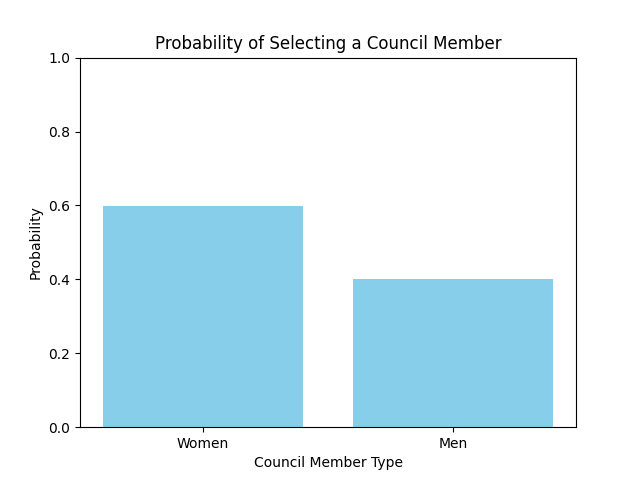
\includegraphics[width=\columnwidth]{figs/fig1.png}
   \end{figure}
\begin{figure}[h!]
   \centering
   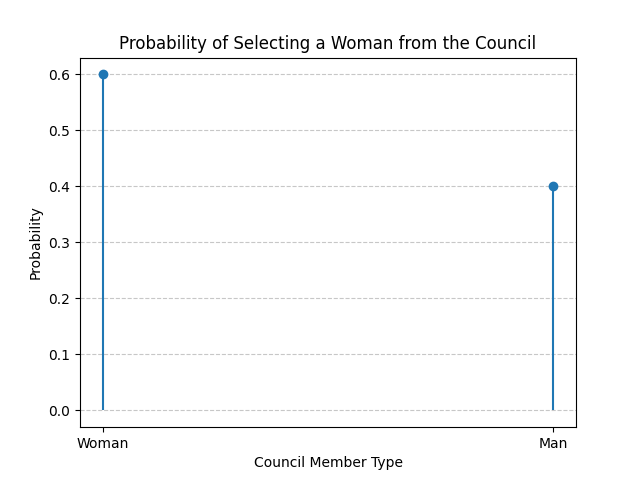
\includegraphics[width=\columnwidth]{figs/fig2.png}
   \end{figure}

\end{document}

